\documentclass[9pt, usenames, dvipsnames]{beamer}
\usetheme{CambridgeUS}
\usecolortheme{beaver}
\useinnertheme{rectangles}
\useoutertheme{smoothbars}

\usepackage[T1]{fontenc}
\usepackage[utf8]{inputenc}
\usepackage{lmodern}
\usepackage{textpos}

\usepackage{pdfpages}
\usepackage[english]{babel}
\usepackage{csquotes}
\usepackage{geometry}
\usepackage{graphicx}
\usepackage{subcaption}
\usepackage{hyperref}
\usepackage{url}
\usepackage{xcolor, colortbl}
\usepackage{amsmath, amssymb, amsfonts}
\usepackage[super]{nth}
\usepackage{fancybox}
\usepackage{lipsum}

\usepackage{tabularx}
\usepackage{longtable}
\usepackage{booktabs}
\usepackage{float}
\usepackage{appendixnumberbeamer}
\restylefloat{table}
\usepackage{array}
\usepackage{tikz}
\usetikzlibrary{arrows.meta, positioning}
\tikzset{%
  >={Latex[width=10mm, length=3mm]},
  base/.style = {rectangle, draw = black, text centered, font = \sffamily, minimum width = 1cm , minimum height = 3cm, text width = 2cm},
  ETF/.style = {base, fill = blue!80},
  AP/.style = {base, fill = blue!60},
  Investor/.style = {base, fill = red!60},
  Exchange/.style = {base, fill = lightgray},
  arrow/.style = {->, shorten >=2pt, width=10mm}
}


\usepackage[backend=biber, dateabbrev=true, citestyle=authoryear-icomp, bibstyle=authoryear-icomp, useprefix=true, language=english]{biblatex}
%\nocite{*}
\bibliography{../Bibliography/BibETF}

\setbeamertemplate{caption}[numbered]
\setbeamertemplate{bibliography item}[text]
\title[ETFs' unintended effects on stocks]{Exchange-traded funds' expansion and their unintended effects over underlying stocks}
\subtitle{Volatility, liquidity and efficiency}
\author{Gr\'egoire Pichard}
\date{\today}
\institute{HEC Lausanne (Unil)}
\subject{Master of Science in Finance (\textsc{MScF})}
%\logo{
\includegraphics[scale = 0.3]{lo_unil_hec06_bleu.eps}}

\setbeamercovered{transparent}
\begin{document}
\begin{frame}
  \titlepage
\end{frame}

\begin{frame}
  \frametitle{All evil rooted in one product ?}
  \shadowbox{\parbox{\textwidth}{\textbf{The Silent Road to Serfdom : Why Passive Investing is Worst Than Marxism} -- Note by I.~Fraser-Jenkins, \emph{Sanford C. Bernstein \& Co.}, 2016}}
  \begin{columns}
    \begin{column}{0.6\textwidth}
      \begin{itemize}
      \item<1-> Abstract : the shift of a growing share of capital markets towards passive, index-based investing prevents the efficient reallocation of capital from overpriced to underpriced companies. Active management and the related research generate positive externalities.
      \item<2-> Are this concern and conclusion justified ?
        \begin{itemize}
        \item What are the author's interests ? This is from the quantitative research of an asset management company, also running retail mutual funds.
        \item {In general:\\
          \begin{quote}
            Everything which is exaggerated is insignificant.\hfill{ \tiny Talleyrand}
        \end{quote}}
        \end{itemize}
      \end{itemize}
    \end{column}
    \begin{column}{0.4\textwidth}
      \begin{figure}
        \fbox{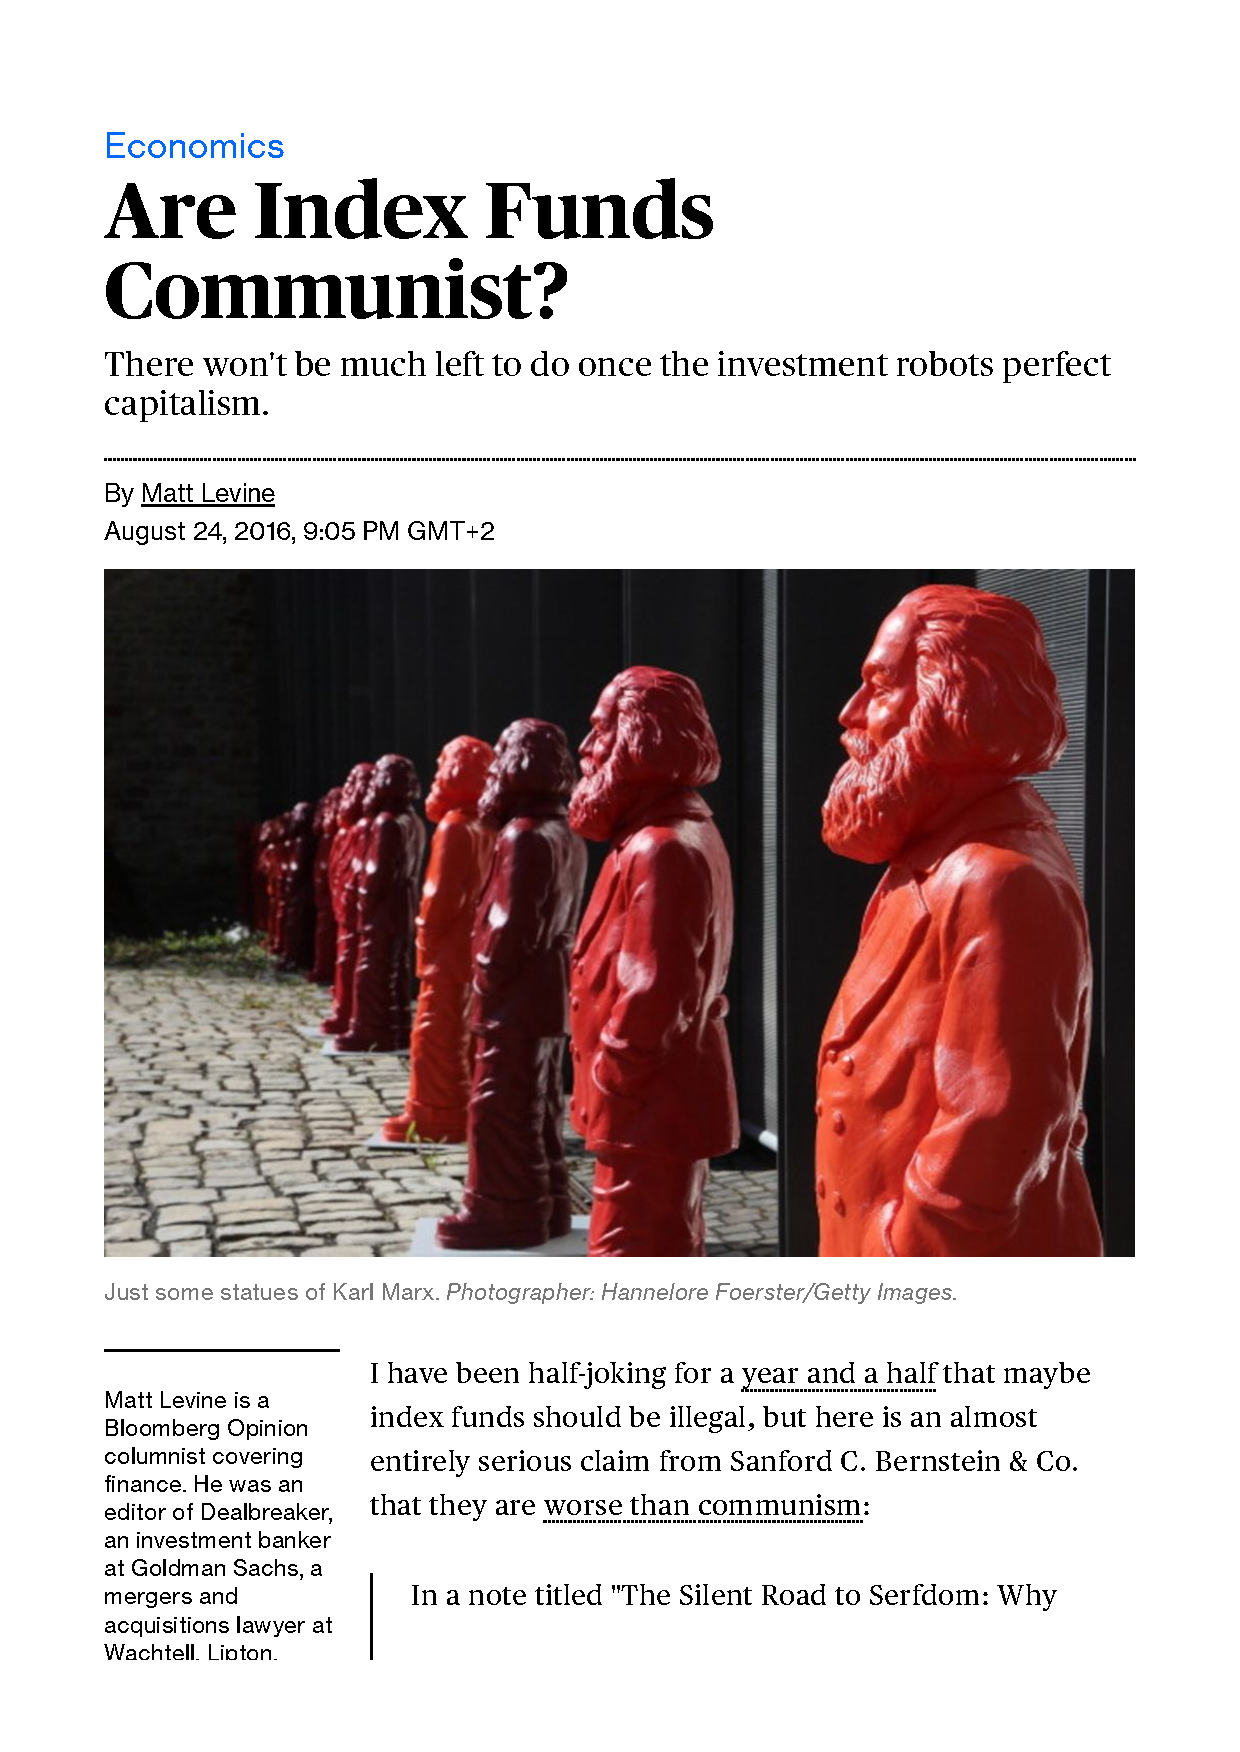
\includegraphics[page=1, width = 0.7\textwidth, height = 1.2\textwidth, keepaspectratio]{ETF_WorstThanMarxism.pdf}}
        \caption{\tiny Matt Levine, Bloomberg Opinion, 24.08.2016, available at: \url{https://www.bloomberg.com/opinion/articles/2016-08-24/are-index-funds-communist\#footnote-1472053794479}}
        \label{fig:Bloomberg_ETFMarxism}
      \end{figure}
    \end{column}
  \end{columns}
\end{frame}

\begin{frame}
  \frametitle{Research field \& focus}
  \begin{block}{General concerns expressed}
    \begin{itemize}
    \item What effects are caused through index-tracking securities and \textbf{especially ETFs} on underlying securities ?
    \item Is there a new risk investors and regulators should become aware of ?
    \end{itemize}
  \end{block}
  \begin{alertblock}{Warning}
    Focusing on observable indicators of the risk and loss of efficiency is needed: choice based on existing research strategies.
  \end{alertblock}
  \begin{exampleblock}{Research questions}
    Three aspects are treated over a broad and long sample of stocks:
    \begin{enumerate}
    \item<1-> Do ETFs increase underlying stocks' volatility over the short term ?
    \item<2-> Do ETFs divert the liquidity and thus decrease it at the individual security level ?
    \item<3-> Are there signs ETFs make prices noisier, hence less efficient ? 
    \end{enumerate}
  \end{exampleblock}
\end{frame}


\begin{frame}
  \frametitle{Outline}
  \tableofcontents
\end{frame}

\section{Context}
\subsection{Exponential growth of a new fund type}
\begin{frame}
  \frametitle{Capitalization worldwide}
  \begin{figure}
    \centering
    \caption{Comparison of total stock market vs. ETF capitalization\footcite[172]{Ben-David2017}}
    \label{fig:Fig1_MarketCap}
    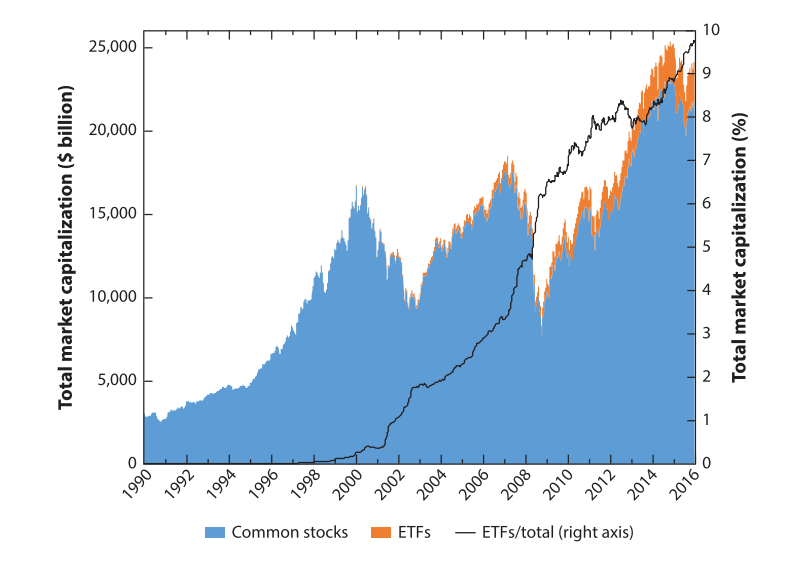
\includegraphics[width = \textwidth, height = 0.65\paperheight, keepaspectratio]{Fig1_MarketCap}
  \end{figure}
\end{frame}


\begin{frame}
  \frametitle{Trading volume, share of total}
  \begin{figure}
    \centering
    \caption{Comparison of total stock market vs. ETF-related daily trading volume\footcite[173]{Ben-David2017}}
    \label{fig:Fig2_Volume}
    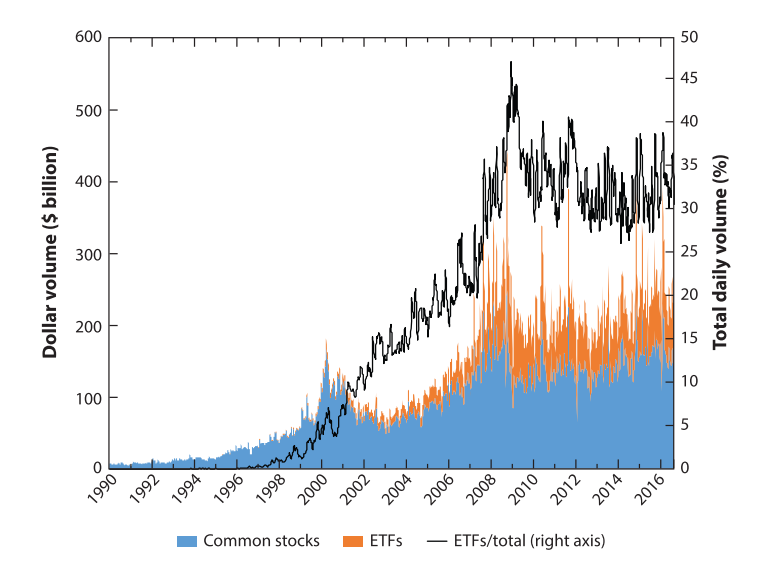
\includegraphics[width = \textwidth, height = 0.65\paperheight, keepaspectratio]{Fig2_Volume}
  \end{figure}
\end{frame}

\begin{frame}
  \frametitle{Entities listed in the U.S.}
  \begin{figure}
    \centering
    \caption{Number of ETFs included over the sample period\footnote{Data from \emph{Eikon} fund screener, only physical- and optimized-replication ETFs listed in the U.S.}}
    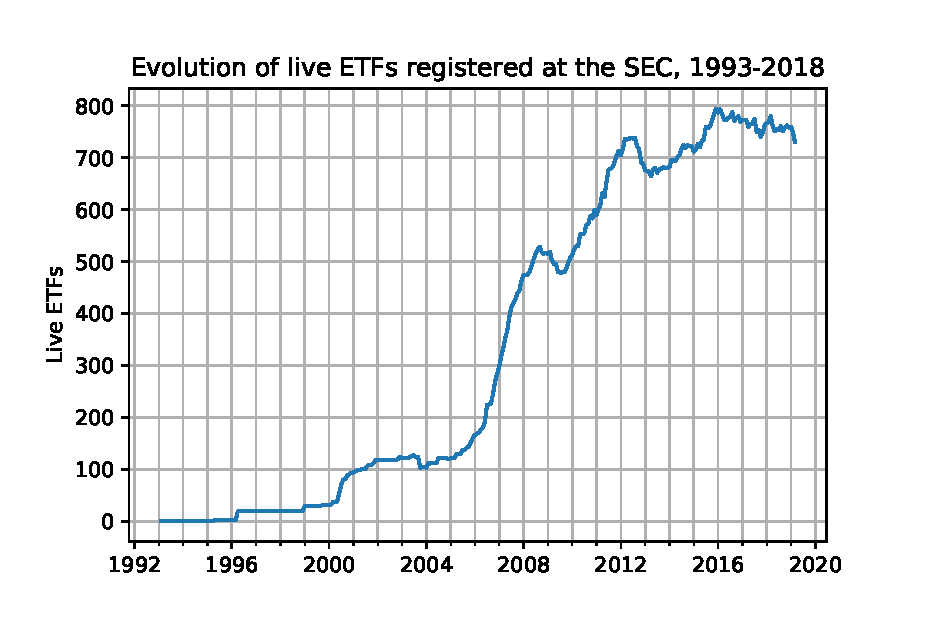
\includegraphics[width = \textwidth, height = 0.65\paperheight, keepaspectratio]{LiveETF_Eikon}
  \end{figure}
\end{frame}

\begin{frame}
  \frametitle{Comparing flows in U.S. equity}
  \begin{figure}
    \centering
    \caption{Shift towards ETF investments and steady outflows from mutual funds}
    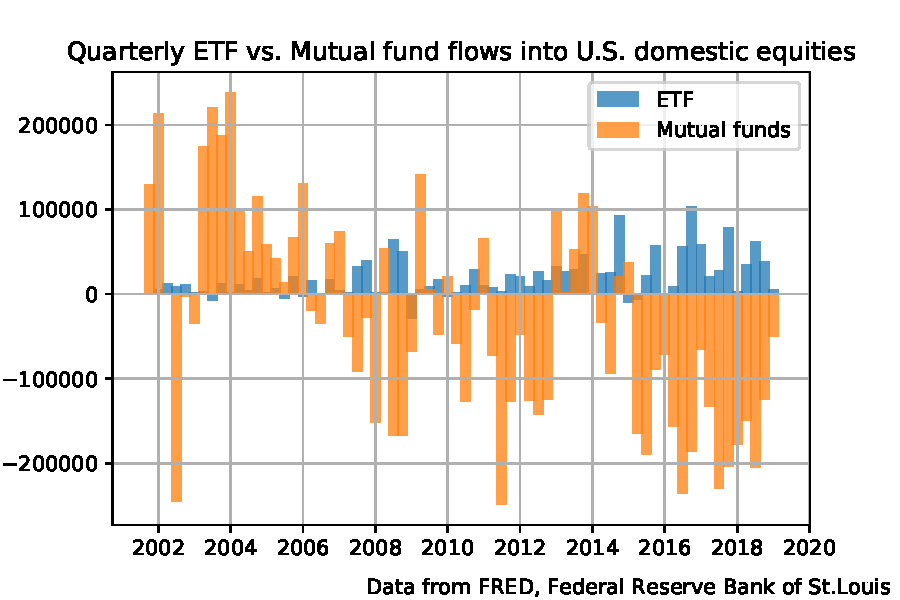
\includegraphics[width = \textwidth, height = 0.65\paperheight, keepaspectratio]{USFlows_ETFvsMutual.pdf}
  \end{figure}
\end{frame}

\subsection{Institutional aspects of ETFs}

\begin{frame}
  \frametitle{Concept and history of exchange-traded funds}
  \begin{itemize}
  \item<1-> Goal at the inception : track a value-weighted equity index using physical replication.
    \begin{itemize}
    \item First ETF ever listed : Toronto Stock Exchange Index Participation Units, introduced March 1990
    \item First ETF listed in the U.S. : State Street SPDR S\&P 500 ETF, a.k.a. ``SPY'', introduced January 1993.
    \item As of June 21, 2019, SPY is the largest ETF by assets under management: USD 266~B.
    \end{itemize}
  \item<2-> A mixture of existing products:
    \begin{itemize}
    \item As (open-end) mutual funds:
      \begin{itemize}
      \item release their Net Asset Value and their holdings
      \item registered as 1940 Act investment companies $\rightarrow$ creation/redemption of shares
      \end{itemize}
    \item As index-funds : track an index built with underlying
      securities and/or derivatives and following rules defined in a
      prospectus
    \item As closed-end funds : traded throughout the day on an
      exchange
    \end{itemize}
  \end{itemize}
  \onslide<3->\begin{alertblock}{Special features}
    \begin{itemize}
    \item the intraday NAV is spread out every 15 seconds, or more often.
    \item \textbf{standardized in-kind or cash creation/redemption process involving authorized participants' arbitrage.}
    \end{itemize}
  \end{alertblock}
\end{frame}

\begin{frame}
  \frametitle{ETF pricing mechanism and trading}
  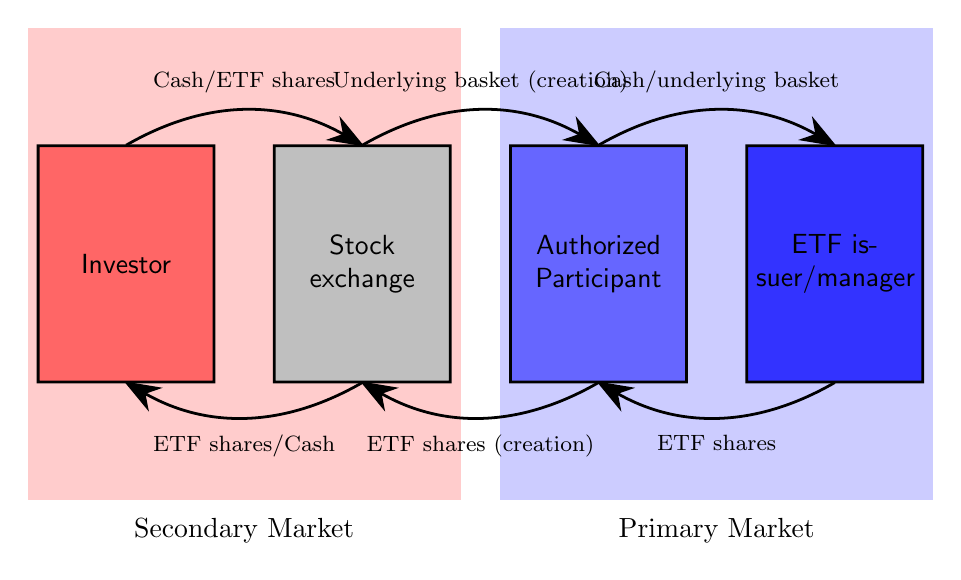
\begin{tikzpicture}[->, >={Stealth[width=3mm, length=4mm]}, auto, node distance=3cm, align = center]
    \node[base, minimum height = 6cm, minimum width = 5.5cm, fill=red!20, draw=none] at (-8.5, 0) (SecMarket) {};
    \node[base, minimum height = 6cm, minimum width = 5.5cm, fill=blue!20, right of=SecMarket, draw = none] at ([xshift=3cm] SecMarket) (PriMarket) {};
    \node[below of=PriMarket, below = 3pt] (PriMarketLabel) {Primary Market};
    \node[below of=SecMarket, below = 3pt] (SecMarketLabel) {Secondary Market};
    \begin{scope}[transparency group]
      \node at (-1,0) (ETF) [ETF] {ETF issuer/manager};
      \node (AP) [AP, left of = ETF] {Authorized Participant};
      \node (Exchange) [Exchange, left of = AP] {Stock exchange};
      \node (Investor) [Investor, left of = Exchange] {Investor};
      \draw[->] (Investor.north) to [out=30, in=150] node[above = 3pt, font=\footnotesize] {Cash/ETF shares} (Exchange.north);
      \draw[->] (Exchange.north) to [out=30, in = 150] node[above = 3pt, font=\footnotesize] {Underlying basket (creation)} (AP.north);
      \draw[->] (AP.north) to [out=30, in = 150] node[above = 3pt, font=\footnotesize] {Cash/underlying basket} (ETF.north);
      \draw[->] (ETF.south) to [in=330, out = 210] node[below = 3pt, font=\footnotesize] {ETF shares} (AP.south);
      \draw[->] (AP.south) to [in=330, out = 210] node[below = 3pt, font=\footnotesize] {ETF shares (creation)} (Exchange.south);
      \draw[->] (Exchange.south) to [in=330, out = 210] node[below = 3pt, font=\footnotesize] {ETF shares/Cash} (Investor.south);
    \end{scope}
  \end{tikzpicture}  
\end{frame}

\subsection{Evidence-based concerns expressed about ETFs}
\begin{frame}
  \frametitle{Concerns expressed about risks conveyed through ETFs}
  \begin{itemize}
  \item Liquidity : apart from idiosyncratic events (e.g. 2010 Flash Crash), ETFs in general are very liquid thanks to the arbitrage mechanism. E.g. \textcite{Ben-David2018} show their turnover is higher than stocks.
  \item What about underlying securities' liquidity ?
  \end{itemize}
  \begin{alertblock}{Under regulatory scrutiny}
    This asset category started to worry regulators less than a decade ago, without leading them to clear conclusions nor actions.
    \begin{quotation}
      [ETFs] may transmit or amplify financial shocks originating elsewhere.

      [\dots]

      ETFs [\dots] could also potentially accelerate or amplify movements in markets during market turbulence, thus reducing market liquidity.\flushright{\footnotesize U.S. Dept. of Treasury, Office of Financial Research, September 2013}
    \end{quotation}
  \end{alertblock}
  
\end{frame}

\begin{frame}[allowframebreaks]
  \frametitle{Selection of academic contributions about ETFs' effects}
  \begin{itemize}
  \item Empirical contributions
    \begin{itemize}
    \item \textcite{Agarwal2017} : quasi-natural experiments with (1) trading halts and (2) Russell indices to show an increase of the \emph{commonality} of stock liquidity with respect to a highly ETF-owned basket of other stocks.
    \item \textcite{Da2018} :
      \begin{itemize}
      \item ETFs' turnover, but not ownership, is positively linked with the comovement of their component stocks.
      \item Stock-level analysis : average turnover of ETF shareholders predictscomovement with the market; mean reversion due to ETF flows and comovement is thus \emph{excessive}
      \end{itemize}
    \item \textcite{Leippold2015} (including a model) : introduction of equity ETF increases the average correlation among index components as well as non-index components, more than index futures did.
    \item \textcite{Krause2014} (idem) : variance spillovers between ETFs and their largest component stocks are positively correlated with liquidity, ETF ownership share, ETF flows and their market capitalization; the relationship strengthens for small stocks.
      %\item \textcite{Petajisto2017} : despite the arbitrage mechanism involving authorized participants, prices of ETFs tracking illiquid securities deviate more from NAV, allowing for active strategies arbitraging mispricing across similar ETFs.
    \end{itemize}
  \item Theoretical models
    \begin{itemize}
    \item \textcite{Bhattacharya2016} : as ETFs provide access to otherwise illiquid securities, ETF-related information distorts those securities' prices. (``tail wagging the dog'' in authors' words)
    \item \textcite{Chinco2016} : ETF rebalancing cause subsequent rebalancing cascades reaching stocks held together in ETF portfolios; the direction of a stock's move is impossible to predict.
    \end{itemize}
  \end{itemize}

  \begin{exampleblock}{Most relevant}
    {\bfseries Part of the methodology} in the following articles has served for this thesis, which replicates and extends their results:
    \begin{itemize}
    \item \textcite{Ben-David2018}
      \begin{itemize}
      \item {\bfseries Monthly volatility impact of ETF ownership} : \emph{liquidity trading hypothesis} vs. \emph{liquidity buffer hypothesis}
      \item Robust IV setting using exogenous index membership changes (Russell 3000)
      \item {\bfseries Reversion of prices after a shock} : \emph{liquidity trading hypothesis} vs. \emph{price discovery hypothesis}
      \item Price impact of ETF flows using trade-level data
      \item Correction of mispricing (arbitrage) and intraday volatility
      \item Asset pricing consequence : a risk premium for the volatility caused by ETF interest.      
      \end{itemize}
    \item \textcite{Israeli2017}
      \begin{itemize}
      \item Testing two hypotheses showing that ETF appeal to noise traders, who migrate from individual securities, while informed traders find less liquidity on underlying stocks.
        \begin{enumerate}
        \item Trading costs increasing with ETF ownership
        \item Deterioration of the informational efficiency of stock prices
        \end{enumerate}
      \item {\bfseries Proxies for liquidity : bid-ask spread estimator and \textcite{Amihud2002} illiquidity ratio}
      \item Proxies for firm-level informational efficiency : return synchronicity, future earnings response and analyst coverage
      \end{itemize}
    \end{itemize}
  \end{exampleblock}
\end{frame}

\subsection{Selection of related research}
\begin{frame}
  \frametitle{Expliciting relevant research : \textcite{Ben-David2018}}
\end{frame}

\begin{frame}
  \frametitle{Expliciting relevant research : \textcite{Israeli2017}}
\end{frame}

\section{Research method and main results}
\subsection{Data}
\begin{frame}
  \frametitle{Data coverage}
  \begin{itemize}
  \item<1-> Period : August 1999 -- December 2018
  \item<2-> Frequency:
    \begin{itemize}
    \item Daily price, volume and VWAP series
    \item Monthly ETF and other fund holdings, and controls
    \item Quarterly resampling for variance ratios (estimation of efficiency effects)
    \end{itemize}
  \item<3-> Analysis performed at stock-level over separate samples:
    \begin{itemize}
    \item on a U.S. stocks sample : 4784 companies
    \item on an international sample of stocks: 16417 companies from Europe (EU25 + EFTA), Canada, Japan, BRICS and emerging countries (Israel, Turkey, South Korea, Hong Kong, Taiwan) 
    \end{itemize}
  \item<4-> Exchange-traded funds :
    \begin{itemize}
    \item 3601 live funds as of 2019 Q1, from the \textit{Lipper} database
    \item Physical or optimized replication only
    \item Countries of incorporation not limited to U.S. :
      \begin{itemize}
      \item Americas (Canada, Mexico, Brazil, Colombia)
      \item Europe (France, Germany, Switzerland, Ireland, Spain, Greece, Sweden, Poland, Russia)
      \item Asia-Pacific (Japan, South Korea, India, Hong Kong, Mainland China, Taiwan, Vietnam, Indonesia, Malaysia, Australia, New Zealand)
      \end{itemize}
    \end{itemize}
    \item<5-> Source : Thomson Reuters \emph{Eikon} platform and API. 
  \end{itemize}
  
\end{frame}

\subsection{ETF ownership and the volatility of underlying stocks}
\begin{frame}
  \frametitle{Methodology}
\begin{equation}
  \mathsf{Volatility}_{i,t} = \beta_{0} + \beta_{1} \mathsf{ETF\_ownership}_{i, t} + B_{C}^{\intercal} \mathsf{Controls}_{i, t} + \alpha_{i} + \gamma_{t} + \epsilon_{i, t}
\end{equation}
  
\end{frame}

\begin{frame}
  \frametitle{Estimation results : U.S.}
  \centering
  {\small\tabcolsep=3pt
\begin{longtable}{>{\bfseries}lcccc}
\multicolumn{5}{r}{\textit{Continued from previous page}}\\
\toprule
& \textbf{Baseline}  & \textbf{Controls + Vol. lags} & \textbf{Inst. o'ship controls} & \textbf{Standardized}  \\
\midrule
\endhead
\caption{U.S. Sample : Exchange-Traded Fund aggregate ownership share and the volatility of underlying securities' daily returns}\\
\label{tab:Volatility:US:Comp}\\
\toprule
& \textbf{Baseline}  & \textbf{Controls +lags} & \textbf{O'ship controls} & \textbf{Standardized}  \\
\midrule
\endfirsthead
\bottomrule
\multicolumn{5}{r}{\textit{Continues on next page}}\\
\endfoot
\bottomrule
\endlastfoot
Intercept                         &       0.2964       &             0.0488            &             0.0494             &        -0.0154         \\
         &      (22.268)      &            (7.1942)           &            (7.2977)            &       (-0.4273)        \\
$\mathbf{PctETF}_{t-1}$            &       0.2470       &             0.0385            &             0.0395             &         0.0081         \\
        &      (8.2542)      &            (5.9800)           &            (6.2940)            &        (6.8269)        \\
$\log(\mathbf{MarketCap}_{t-1})$    &      -0.0127       &            -0.0018            &            -0.0018             &        -0.0102         \\
         &     (-20.751)      &           (-5.8479)           &           (-5.9701)            &       (-6.1991)        \\
$1/\mathbf{Close}_{t-1}$                    &       0.0988       &             0.0251            &             0.0251             &         0.1452         \\
            &      (10.972)      &            (7.7261)           &            (7.7792)            &        (7.9151)        \\
$\left(BE/ME\right)_{t-1}$           &     5.552e-07      &           7.393e-07           &           1.038e-06            &       5.019e-06        \\
            &      (2.3023)      &            (4.1534)           &            (8.5166)            &        (5.3019)        \\
$\mathbf{Past 12 to 1M ret.}_{t-1}$               &      -0.0003       &            -0.0004            &            -0.0004             &        -0.0024   \\
&     (-0.6844)      &           (-1.8758)           &           (-1.8564)            &       (-1.8927)        \\
$\mathbf{AmihudRatio}_{t-1}$                 &                    &             3.4590            &             3.4611             &         19.952         \\
        &                    &            (2.7034)           &            (2.7029)            &        (2.7038)        \\
$\mathbf{BidAskSpread}_{t-1}$             &                    &             0.1750            &             0.1748             &         1.0060         \\
 &                    &            (4.5505)           &            (4.5446)            &        (4.5471)        \\
$\mathbf{G.Profit.}_{t-1}$          &                    &            -0.0005            &            -0.0005             &        -0.0028         \\
            &                    &           (-2.6218)           &           (-2.6334)            &       (-2.6197)        \\
$\mathbf{Volatility}_{t-1}$                  &                    &             0.1377            &             0.1378             &         0.1376         \\
       &                    &            (6.7584)           &            (6.7701)            &        (6.7630)        \\
$\mathbf{Volatility}_{t-2}$                  &                    &             0.1605            &             0.1604             &         0.1603         \\
                &                    &            (16.002)           &            (15.972)            &        (15.949)        \\
$\mathbf{Volatility}_{t-3}$                  &                    &             0.1230            &             0.1229             &         0.1229         \\
                            &                    &            (13.390)           &            (13.402)            &        (13.403)        \\
$\mathbf{Volatility}_{t-4}$                  &                    &             0.0819            &             0.0818             &         0.0817         \\
                 &                    &            (9.8851)           &            (9.8688)            &        (9.8756)        \\
$\mathbf{PctOtherMutual}_{t-1}$    &                    &                               &            -0.0003             &        -0.0016         \\
                       &                    &                               &           (-2.5676)            &       (-1.1497)        \\
$\mathbf{PctPension}_{t-1}$        &                    &                               &             1.0330             &         0.0015         \\
                               &                    &                               &            (3.4034)            &        (3.6451)        \\
$\mathbf{PctHedge}_{t-1}$          &                    &                               &            -0.0284             &       9.023e-05        \\
                           &                    &                               &           (-3.2527)            &        (0.4613)        \\
\midrule
Effects                           &       Entity       &             Entity            &             Entity             &         Entity         \\
& Time &  Time  &  Time &  Time\\
\bottomrule
\pagebreak
\toprule
& \textbf{Baseline}  & \textbf{Controls +lags} & \textbf{O'ship controls} & \textbf{Standardized}  \\
\midrule
Dep. Variable                     &     Volatility     &           Volatility          &           Volatility           &       Volatility       \\
Estimator                         &      PanelOLS      &            PanelOLS           &            PanelOLS            &        PanelOLS        \\
No. Observations                  &       413304       &             297405            &             297399             &         297247         \\
Cov. Est.                         &   Driscoll-Kraay   &         Driscoll-Kraay        &         Driscoll-Kraay         &     Driscoll-Kraay     \\
$R^{2}$                         &       0.0545       &             0.1592            &             0.1593             &         0.1594         \\
$R^{2}$ (Within)                &       0.0565       &             0.1353            &             0.1351             &         0.1348         \\
$R^{2}$ (Between)               &       0.2009       &             0.7626            &             0.7625             &         0.7616         \\
$R^{2}$ (Overall)               &       0.1515       &             0.2716            &             0.2715             &         0.2710         \\
F-statistic                       &       4717.9       &             4643.9            &             3718.4             &         3718.6         \\
P-value (F-stat)                  &       0.0000       &             0.0000            &             0.0000             &         0.0000         \\
\bottomrule
\end{longtable}
}

\end{frame}

\begin{frame}
  \frametitle{Estimation results : International}
  \centering
  {\small\tabcolsep=3pt
\begin{longtable}{>{\bfseries}lcccc}
\multicolumn{5}{r}{\textit{Continued from previous page}}\\
\toprule
& \textbf{Baseline}  & \textbf{Controls + Vol. lags} & \textbf{Inst. o'ship controls} & \textbf{Standardized}  \\
\midrule
\endhead
\caption{U.S. Sample : Exchange-Traded Fund aggregate ownership share and the volatility of underlying securities' daily returns}\\
\label{tab:Volatility:US:Comp}\\
\toprule
& \textbf{Baseline}  & \textbf{Controls +lags} & \textbf{O'ship controls} & \textbf{Standardized}  \\
\midrule
\endfirsthead
\bottomrule
\multicolumn{5}{r}{\textit{Continues on next page}}\\
\endfoot
\bottomrule
\endlastfoot
Intercept                         &       0.2964       &             0.0488            &             0.0494             &        -0.0154         \\
         &      (22.268)      &            (7.1942)           &            (7.2977)            &       (-0.4273)        \\
$\mathbf{PctETF}_{t-1}$            &       0.2470       &             0.0385            &             0.0395             &         0.0081         \\
        &      (8.2542)      &            (5.9800)           &            (6.2940)            &        (6.8269)        \\
$\log(\mathbf{MarketCap}_{t-1})$    &      -0.0127       &            -0.0018            &            -0.0018             &        -0.0102         \\
         &     (-20.751)      &           (-5.8479)           &           (-5.9701)            &       (-6.1991)        \\
$1/\mathbf{Close}_{t-1}$                    &       0.0988       &             0.0251            &             0.0251             &         0.1452         \\
            &      (10.972)      &            (7.7261)           &            (7.7792)            &        (7.9151)        \\
$\left(BE/ME\right)_{t-1}$           &     5.552e-07      &           7.393e-07           &           1.038e-06            &       5.019e-06        \\
            &      (2.3023)      &            (4.1534)           &            (8.5166)            &        (5.3019)        \\
$\mathbf{Past 12 to 1M ret.}_{t-1}$               &      -0.0003       &            -0.0004            &            -0.0004             &        -0.0024   \\
&     (-0.6844)      &           (-1.8758)           &           (-1.8564)            &       (-1.8927)        \\
$\mathbf{AmihudRatio}_{t-1}$                 &                    &             3.4590            &             3.4611             &         19.952         \\
        &                    &            (2.7034)           &            (2.7029)            &        (2.7038)        \\
$\mathbf{BidAskSpread}_{t-1}$             &                    &             0.1750            &             0.1748             &         1.0060         \\
 &                    &            (4.5505)           &            (4.5446)            &        (4.5471)        \\
$\mathbf{G.Profit.}_{t-1}$          &                    &            -0.0005            &            -0.0005             &        -0.0028         \\
            &                    &           (-2.6218)           &           (-2.6334)            &       (-2.6197)        \\
$\mathbf{Volatility}_{t-1}$                  &                    &             0.1377            &             0.1378             &         0.1376         \\
       &                    &            (6.7584)           &            (6.7701)            &        (6.7630)        \\
$\mathbf{Volatility}_{t-2}$                  &                    &             0.1605            &             0.1604             &         0.1603         \\
                &                    &            (16.002)           &            (15.972)            &        (15.949)        \\
$\mathbf{Volatility}_{t-3}$                  &                    &             0.1230            &             0.1229             &         0.1229         \\
                            &                    &            (13.390)           &            (13.402)            &        (13.403)        \\
$\mathbf{Volatility}_{t-4}$                  &                    &             0.0819            &             0.0818             &         0.0817         \\
                 &                    &            (9.8851)           &            (9.8688)            &        (9.8756)        \\
$\mathbf{PctOtherMutual}_{t-1}$    &                    &                               &            -0.0003             &        -0.0016         \\
                       &                    &                               &           (-2.5676)            &       (-1.1497)        \\
$\mathbf{PctPension}_{t-1}$        &                    &                               &             1.0330             &         0.0015         \\
                               &                    &                               &            (3.4034)            &        (3.6451)        \\
$\mathbf{PctHedge}_{t-1}$          &                    &                               &            -0.0284             &       9.023e-05        \\
                           &                    &                               &           (-3.2527)            &        (0.4613)        \\
\midrule
Effects                           &       Entity       &             Entity            &             Entity             &         Entity         \\
& Time &  Time  &  Time &  Time\\
\bottomrule
\pagebreak
\toprule
& \textbf{Baseline}  & \textbf{Controls +lags} & \textbf{O'ship controls} & \textbf{Standardized}  \\
\midrule
Dep. Variable                     &     Volatility     &           Volatility          &           Volatility           &       Volatility       \\
Estimator                         &      PanelOLS      &            PanelOLS           &            PanelOLS            &        PanelOLS        \\
No. Observations                  &       413304       &             297405            &             297399             &         297247         \\
Cov. Est.                         &   Driscoll-Kraay   &         Driscoll-Kraay        &         Driscoll-Kraay         &     Driscoll-Kraay     \\
$R^{2}$                         &       0.0545       &             0.1592            &             0.1593             &         0.1594         \\
$R^{2}$ (Within)                &       0.0565       &             0.1353            &             0.1351             &         0.1348         \\
$R^{2}$ (Between)               &       0.2009       &             0.7626            &             0.7625             &         0.7616         \\
$R^{2}$ (Overall)               &       0.1515       &             0.2716            &             0.2715             &         0.2710         \\
F-statistic                       &       4717.9       &             4643.9            &             3718.4             &         3718.6         \\
P-value (F-stat)                  &       0.0000       &             0.0000            &             0.0000             &         0.0000         \\
\bottomrule
\end{longtable}
}

\end{frame}

\subsection{ETF ownership and the liquidity of underlying stocks}
\begin{frame}
  \frametitle{Methodology}
  \begin{equation}
 \mathsf{PctBidAskSpread}_{i,t} = \beta_{0} + \beta_{1} \mathsf{ETF\_ownership}_{i, t - 1} + B_{C}^{\intercal} \mathsf{Controls}_{i, t - 1} + \alpha_{i} + \gamma_{t} + \epsilon_{i, t}
  \end{equation}

  \begin{equation}
   \mathsf{Illiq^{Num}}_{i,t} = \beta_{0} + \beta_{1} \mathsf{ETF\_ownership}_{i, t - 1} + \beta_{2} \mathsf{Illiq^{Denom}_{i,t}} + B_{C}^{\intercal} \mathsf{Controls}_{i, t- 1} + \alpha_{i} + \gamma_{t} + \epsilon_{i, t}
\end{equation}

\end{frame}

\begin{frame}
  \frametitle{Estimation results : U.S.}
  \centering
  \begin{center}
  \caption{Exchange-Traded Funds' aggregate ownership share and underlying securities' liquidity}
  \label{tab:Liquidity:Comp}
\begin{tabular}{lcccc}
\toprule
                                           &   \textbf{Amihud}   & \textbf{Amihud w/inst. o'ship} &   \textbf{Bid-Ask}  & \textbf{Bid-Ask w/inst. o'ship}  \\
\midrule
\textbf{Dep. Variable}                     &   AmihudNumerator   &        AmihudNumerator         &   PctBidAskSpread   &         PctBidAskSpread          \\
\textbf{Estimator}                         &       PanelOLS      &            PanelOLS            &       PanelOLS      &             PanelOLS             \\
\textbf{No. Observations}                  &        436857       &             436852             &        335350       &              335346              \\
\textbf{Cov. Est.}                         &    Driscoll-Kraay   &         Driscoll-Kraay         &    Driscoll-Kraay   &          Driscoll-Kraay          \\
\textbf{R-squared}                         &        0.0330       &             0.0330             &        0.0512       &              0.0512              \\
\textbf{R-Squared (Within)}                &        0.0436       &             0.0436             &        0.0661       &              0.0663              \\
\textbf{R-Squared (Between)}               &        0.1873       &             0.1873             &        0.5612       &              0.5618              \\
\textbf{R-Squared (Overall)}               &        0.1276       &             0.1276             &        0.1882       &              0.1885              \\
\textbf{F-statistic}                       &        3688.0       &             2950.4             &        4465.5       &              2555.6              \\
\textbf{P-value (F-stat)}                  &        0.0000       &             0.0000             &        0.0000       &              0.0000              \\
\midrule
\textbf{Intercept}                         &        0.3438       &             0.3438             &        0.1054       &              0.1057              \\
\textbf{ }                                 &       (30.192)      &            (30.164)            &       (15.787)      &             (15.743)             \\
\textbf{PctSharesHeldETF}                  &        0.1870       &             0.1871             &        0.0061       &              0.0060              \\
\textbf{ }                                 &       (7.7614)      &            (7.7638)            &       (0.7923)      &             (0.7832)             \\
\textbf{np.log(CompanyMarketCap\_1lag)}    &       -0.0153       &            -0.0153             &       -0.0049       &             -0.0049              \\
\textbf{ }                                 &      (-26.847)      &           (-26.822)            &      (-14.639)      &            (-14.596)             \\
\textbf{BookToMarketRatio\_1lag}           &      2.894e-07      &           3.098e-07            &      -4.277e-08     &            -4.038e-08            \\
\textbf{ }                                 &       (1.1320)      &            (1.1432)            &      (-0.9008)      &            (-0.8852)             \\
\textbf{AmihudDenominator}                 &      1.321e-11      &            1.32e-11            &                     &                                  \\
\textbf{ }                                 &       (4.1972)      &            (4.1968)            &                     &                                  \\
\textbf{PctSharesHeldOtherMutual}          &                     &           -1.219e-05           &                     &            -2.114e-06            \\
\textbf{ }                                 &                     &           (-5.6177)            &                     &            (-4.5245)             \\
\textbf{Volatility\_1lag}                  &                     &                                &        0.0500       &              0.0499              \\
\textbf{ }                                 &                     &                                &       (10.104)      &             (10.107)             \\
\textbf{PctSharesHeldPension}              &                     &                                &                     &              0.3943              \\
\textbf{ }                                 &                     &                                &                     &             (1.2835)             \\
\textbf{PctSharesHeldHedge}                &                     &                                &                     &              0.0077              \\
\textbf{ }                                 &                     &                                &                     &             (1.7387)             \\
\midrule
\textbf{Effects}                           &        Entity       &             Entity             &        Entity       &              Entity              \\
& Time & Time & Time & Time\\
\bottomrule
\end{tabular}
\end{center}

T-stats reported in parentheses

\end{frame}

\begin{frame}
  \frametitle{Estimation results : International}
  \centering
  \begin{center}
  \caption{Exchange-Traded Funds' aggregate ownership share and underlying securities' liquidity}
  \label{tab:Liquidity:Comp}
\begin{tabular}{lcccc}
\toprule
                                           &   \textbf{Amihud}   & \textbf{Amihud w/inst. o'ship} &   \textbf{Bid-Ask}  & \textbf{Bid-Ask w/inst. o'ship}  \\
\midrule
\textbf{Dep. Variable}                     &   AmihudNumerator   &        AmihudNumerator         &   PctBidAskSpread   &         PctBidAskSpread          \\
\textbf{Estimator}                         &       PanelOLS      &            PanelOLS            &       PanelOLS      &             PanelOLS             \\
\textbf{No. Observations}                  &        436857       &             436852             &        335350       &              335346              \\
\textbf{Cov. Est.}                         &    Driscoll-Kraay   &         Driscoll-Kraay         &    Driscoll-Kraay   &          Driscoll-Kraay          \\
\textbf{R-squared}                         &        0.0330       &             0.0330             &        0.0512       &              0.0512              \\
\textbf{R-Squared (Within)}                &        0.0436       &             0.0436             &        0.0661       &              0.0663              \\
\textbf{R-Squared (Between)}               &        0.1873       &             0.1873             &        0.5612       &              0.5618              \\
\textbf{R-Squared (Overall)}               &        0.1276       &             0.1276             &        0.1882       &              0.1885              \\
\textbf{F-statistic}                       &        3688.0       &             2950.4             &        4465.5       &              2555.6              \\
\textbf{P-value (F-stat)}                  &        0.0000       &             0.0000             &        0.0000       &              0.0000              \\
\midrule
\textbf{Intercept}                         &        0.3438       &             0.3438             &        0.1054       &              0.1057              \\
\textbf{ }                                 &       (30.192)      &            (30.164)            &       (15.787)      &             (15.743)             \\
\textbf{PctSharesHeldETF}                  &        0.1870       &             0.1871             &        0.0061       &              0.0060              \\
\textbf{ }                                 &       (7.7614)      &            (7.7638)            &       (0.7923)      &             (0.7832)             \\
\textbf{np.log(CompanyMarketCap\_1lag)}    &       -0.0153       &            -0.0153             &       -0.0049       &             -0.0049              \\
\textbf{ }                                 &      (-26.847)      &           (-26.822)            &      (-14.639)      &            (-14.596)             \\
\textbf{BookToMarketRatio\_1lag}           &      2.894e-07      &           3.098e-07            &      -4.277e-08     &            -4.038e-08            \\
\textbf{ }                                 &       (1.1320)      &            (1.1432)            &      (-0.9008)      &            (-0.8852)             \\
\textbf{AmihudDenominator}                 &      1.321e-11      &            1.32e-11            &                     &                                  \\
\textbf{ }                                 &       (4.1972)      &            (4.1968)            &                     &                                  \\
\textbf{PctSharesHeldOtherMutual}          &                     &           -1.219e-05           &                     &            -2.114e-06            \\
\textbf{ }                                 &                     &           (-5.6177)            &                     &            (-4.5245)             \\
\textbf{Volatility\_1lag}                  &                     &                                &        0.0500       &              0.0499              \\
\textbf{ }                                 &                     &                                &       (10.104)      &             (10.107)             \\
\textbf{PctSharesHeldPension}              &                     &                                &                     &              0.3943              \\
\textbf{ }                                 &                     &                                &                     &             (1.2835)             \\
\textbf{PctSharesHeldHedge}                &                     &                                &                     &              0.0077              \\
\textbf{ }                                 &                     &                                &                     &             (1.7387)             \\
\midrule
\textbf{Effects}                           &        Entity       &             Entity             &        Entity       &              Entity              \\
& Time & Time & Time & Time\\
\bottomrule
\end{tabular}
\end{center}

T-stats reported in parentheses

\end{frame}


\subsection{ETF ownership and the price efficiency of underlying stocks}
\begin{frame}
  \frametitle{Methodology}
  
\begin{equation}
  VR_{iq} = \beta_{0} + \beta_{1} \mathsf{ETF\_ownership}_{i, q - 1} + B_{C}^{\intercal} \mathsf{Controls}_{i, q - 1} + \alpha_{i} + \gamma_{q} + \epsilon_{i, q}
\end{equation}

\begin{equation}
 absVR_{iq} = \beta_{0} + \beta_{1} \mathsf{ETF\_ownership}_{i, q - 1} + B_{C}^{\intercal} \mathsf{Controls}_{i, q - 1} + \alpha_{i} + \gamma_{q} + \epsilon_{i, q}
\end{equation}

\end{frame}

\begin{frame}
  \frametitle{Estimation results : U.S.}
  \centering
  \begin{center}
  \caption{U.S. Sample : Exchange-Traded Funds' aggregate ownership share and weekly mean reversion of underlying securities}
  \label{tab:Efficiency:US:Comp}
  \begin{tabular}{lcccc}
\toprule
                                           &  \textbf{Abs. VR}  & \textbf{Abs. VR w/inst. o'ship} &    \textbf{VR}     & \textbf{VR w/inst. o'ship}  \\
\midrule
\textbf{Dep. Variable}                     &       absVR        &              absVR              &         VR         &             VR              \\
\textbf{Estimator}                         &      PanelOLS      &             PanelOLS            &      PanelOLS      &          PanelOLS           \\
\textbf{No. Observations}                  &       126851       &              126847             &       126851       &           126847            \\
\textbf{Cov. Est.}                         &   Driscoll-Kraay   &          Driscoll-Kraay         &   Driscoll-Kraay   &       Driscoll-Kraay        \\
\textbf{R-squared}                         &       0.0079       &              0.0081             &       0.0040       &           0.0041            \\
\textbf{R-Squared (Within)}                &       0.0106       &              0.0106             &       0.0040       &           0.0042            \\
\textbf{R-Squared (Between)}               &       0.2814       &              0.2820             &       0.1376       &           0.1385            \\
\textbf{R-Squared (Overall)}               &       0.0318       &              0.0320             &       0.0163       &           0.0165            \\
\textbf{F-statistic}                       &       123.79       &              91.734             &       61.843       &           46.323            \\
\textbf{P-value (F-stat)}                  &       0.0000       &              0.0000             &       0.0000       &           0.0000            \\
\midrule
\textbf{Intercept}                         &       0.8523       &              0.8532             &       0.8735       &           0.8579            \\
\textbf{ }                                 &      (12.280)      &             (12.208)            &      (7.6512)      &          (7.4328)           \\
\textbf{PctSharesHeldETF\_1lag}            &       0.0096       &              0.0218             &      -0.1205       &          -0.1005            \\
\textbf{ }                                 &      (0.1484)      &             (0.3373)            &     (-1.4081)      &         (-1.1660)           \\
\textbf{np.log(CompanyMarketCap\_1lag)}    &      -0.0248       &             -0.0248             &       0.0044       &           0.0052            \\
\textbf{ }                                 &     (-7.5202)      &            (-7.4640)            &      (0.8038)      &          (0.9458)           \\
\textbf{InvClose\_1lag}                    &       0.1276       &              0.1277             &      -0.2002       &          -0.1986            \\
\textbf{ }                                 &      (5.5223)      &             (5.5778)            &     (-6.0619)      &         (-5.9225)           \\
\textbf{AmihudRatio\_1lag}                 &       9.9267       &              9.9488             &      -15.135       &          -15.117            \\
\textbf{ }                                 &      (3.1431)      &             (3.1455)            &     (-3.0288)      &         (-3.0279)           \\
\textbf{PctBidAskSpread\_1lag}             &       0.9314       &              0.9286             &      -1.2190       &          -1.2179            \\
\textbf{ }                                 &      (5.5878)      &             (5.6027)            &     (-3.5732)      &         (-3.5633)           \\
\textbf{BookToMarketRatio\_1lag}           &     -3.498e-06     &            4.433e-05            &     -1.257e-05     &         6.777e-05           \\
\textbf{ }                                 &     (-0.5195)      &             (3.9695)            &     (-1.4303)      &          (3.2826)           \\
\textbf{RetPast12to7M\_1lag}               &       0.0003       &            -9.153e-05           &      -0.0006       &          -0.0013            \\
\textbf{ }                                 &      (0.5981)      &            (-0.2511)            &     (-0.9013)      &         (-2.2311)           \\
\textbf{GrossProfitability\_1lag}          &       0.0011       &              0.0012             &       0.0064       &           0.0062            \\
\textbf{ }                                 &      (0.2252)      &             (0.2454)            &      (1.2767)      &          (1.2635)           \\
\textbf{PctSharesHeldOtherMutual\_1lag}    &                    &             -0.0053             &                    &          -0.0086            \\
\textbf{ }                                 &                    &            (-3.9260)            &                    &         (-3.6908)           \\
\textbf{PctSharesHeldPension\_1lag}        &                    &              11.292             &                    &          -3.7029            \\
\textbf{ }                                 &                    &             (4.1468)            &                    &         (-0.5362)           \\
\textbf{PctSharesHeldHedge\_1lag}          &                    &             -0.1294             &                    &          -0.1145            \\
\textbf{ }                                 &                    &            (-0.8927)            &                    &         (-0.6268)           \\
\midrule
\textbf{Effects}                           &       Entity       &              Entity             &       Entity       &           Entity            \\
& Time & Time & Time & Time\\
\bottomrule
\end{tabular}
\end{center}
T-stats reported in parentheses.

\end{frame}

\begin{frame}
  \frametitle{Estimation results : International}
  \centering
  \begin{center}
  \caption{U.S. Sample : Exchange-Traded Funds' aggregate ownership share and weekly mean reversion of underlying securities}
  \label{tab:Efficiency:US:Comp}
  \begin{tabular}{lcccc}
\toprule
                                           &  \textbf{Abs. VR}  & \textbf{Abs. VR w/inst. o'ship} &    \textbf{VR}     & \textbf{VR w/inst. o'ship}  \\
\midrule
\textbf{Dep. Variable}                     &       absVR        &              absVR              &         VR         &             VR              \\
\textbf{Estimator}                         &      PanelOLS      &             PanelOLS            &      PanelOLS      &          PanelOLS           \\
\textbf{No. Observations}                  &       126851       &              126847             &       126851       &           126847            \\
\textbf{Cov. Est.}                         &   Driscoll-Kraay   &          Driscoll-Kraay         &   Driscoll-Kraay   &       Driscoll-Kraay        \\
\textbf{R-squared}                         &       0.0079       &              0.0081             &       0.0040       &           0.0041            \\
\textbf{R-Squared (Within)}                &       0.0106       &              0.0106             &       0.0040       &           0.0042            \\
\textbf{R-Squared (Between)}               &       0.2814       &              0.2820             &       0.1376       &           0.1385            \\
\textbf{R-Squared (Overall)}               &       0.0318       &              0.0320             &       0.0163       &           0.0165            \\
\textbf{F-statistic}                       &       123.79       &              91.734             &       61.843       &           46.323            \\
\textbf{P-value (F-stat)}                  &       0.0000       &              0.0000             &       0.0000       &           0.0000            \\
\midrule
\textbf{Intercept}                         &       0.8523       &              0.8532             &       0.8735       &           0.8579            \\
\textbf{ }                                 &      (12.280)      &             (12.208)            &      (7.6512)      &          (7.4328)           \\
\textbf{PctSharesHeldETF\_1lag}            &       0.0096       &              0.0218             &      -0.1205       &          -0.1005            \\
\textbf{ }                                 &      (0.1484)      &             (0.3373)            &     (-1.4081)      &         (-1.1660)           \\
\textbf{np.log(CompanyMarketCap\_1lag)}    &      -0.0248       &             -0.0248             &       0.0044       &           0.0052            \\
\textbf{ }                                 &     (-7.5202)      &            (-7.4640)            &      (0.8038)      &          (0.9458)           \\
\textbf{InvClose\_1lag}                    &       0.1276       &              0.1277             &      -0.2002       &          -0.1986            \\
\textbf{ }                                 &      (5.5223)      &             (5.5778)            &     (-6.0619)      &         (-5.9225)           \\
\textbf{AmihudRatio\_1lag}                 &       9.9267       &              9.9488             &      -15.135       &          -15.117            \\
\textbf{ }                                 &      (3.1431)      &             (3.1455)            &     (-3.0288)      &         (-3.0279)           \\
\textbf{PctBidAskSpread\_1lag}             &       0.9314       &              0.9286             &      -1.2190       &          -1.2179            \\
\textbf{ }                                 &      (5.5878)      &             (5.6027)            &     (-3.5732)      &         (-3.5633)           \\
\textbf{BookToMarketRatio\_1lag}           &     -3.498e-06     &            4.433e-05            &     -1.257e-05     &         6.777e-05           \\
\textbf{ }                                 &     (-0.5195)      &             (3.9695)            &     (-1.4303)      &          (3.2826)           \\
\textbf{RetPast12to7M\_1lag}               &       0.0003       &            -9.153e-05           &      -0.0006       &          -0.0013            \\
\textbf{ }                                 &      (0.5981)      &            (-0.2511)            &     (-0.9013)      &         (-2.2311)           \\
\textbf{GrossProfitability\_1lag}          &       0.0011       &              0.0012             &       0.0064       &           0.0062            \\
\textbf{ }                                 &      (0.2252)      &             (0.2454)            &      (1.2767)      &          (1.2635)           \\
\textbf{PctSharesHeldOtherMutual\_1lag}    &                    &             -0.0053             &                    &          -0.0086            \\
\textbf{ }                                 &                    &            (-3.9260)            &                    &         (-3.6908)           \\
\textbf{PctSharesHeldPension\_1lag}        &                    &              11.292             &                    &          -3.7029            \\
\textbf{ }                                 &                    &             (4.1468)            &                    &         (-0.5362)           \\
\textbf{PctSharesHeldHedge\_1lag}          &                    &             -0.1294             &                    &          -0.1145            \\
\textbf{ }                                 &                    &            (-0.8927)            &                    &         (-0.6268)           \\
\midrule
\textbf{Effects}                           &       Entity       &              Entity             &       Entity       &           Entity            \\
& Time & Time & Time & Time\\
\bottomrule
\end{tabular}
\end{center}
T-stats reported in parentheses.

\end{frame}

\section{Conclusion}
\subsection{Wrap-up}

\begin{frame}
  \frametitle{Key findings}
  \begin{itemize}
  \item On average, the volatility of U.S. stocks rises with the share of their equity held by ETFs.
  \item If the mean reversion also increased because of ETFs, this volatility would be non-fundamental and the \emph{liquidity trading hypothesis} would hold.
  \item \textbf{But no significant effect has been found on U.S. variance ratios.}
  \item Price discovery hypothesis ?
  \end{itemize}
\end{frame}

\subsection{Limitations and further directions}

\begin{frame}[allowframebreaks]
  \frametitle{Likely trends in the ETF universe}
  \begin{itemize}
  \item More active bets, nicknamed \textit{passive-aggressive}
  \item Opaque holdings structures are at an advanced stage in the regulatory approval process in the U.S. (late spring 2019)
    
  \end{itemize}
  \begin{block}{The Precidian model}
    \shadowbox{\parbox{0.9\textwidth}{\textbf{An ETF That Hides Its Secret Sauce Is Poised for Regulator's Nod} -- Bloomberg News, April 8, 2019.\footnote{Available at \url{https://www.bloomberg.com/news/articles/2019-04-08/an-etf-that-hides-its-secret-sauce-is-poised-for-regulator-s-nod}}}}
    \begin{itemize}
    \item Positive signs that the Securities and Exchange Commission will allow the design.
    \item Trading permission is the next decision needed before the product is issued.
    \item Disagreement at the SEC and skepticism from some analysts regarding appeal to investors; reality check needed and \textit{evidence so far has shown that \textcolor{red}{awareness about ETFs can take time}}.
    \end{itemize}
    
  \end{block}
  
\end{frame}


\begin{frame}
  \frametitle{Bibliography}
  \printbibliography
\end{frame}
\appendix
\section{Regression results}
\subsection{Volatility}
\subsubsection{United States}
\begin{frame}[allowframebreaks, t]
  \frametitle{Volatility -- U.S. sample}
  \centering
  {\small\tabcolsep=3pt
\begin{longtable}{>{\bfseries}lcccc}
\multicolumn{5}{r}{\textit{Continued from previous page}}\\
\toprule
& \textbf{Baseline}  & \textbf{Controls + Vol. lags} & \textbf{Inst. o'ship controls} & \textbf{Standardized}  \\
\midrule
\endhead
\caption{U.S. Sample : Exchange-Traded Fund aggregate ownership share and the volatility of underlying securities' daily returns}\\
\label{tab:Volatility:US:Comp}\\
\toprule
& \textbf{Baseline}  & \textbf{Controls +lags} & \textbf{O'ship controls} & \textbf{Standardized}  \\
\midrule
\endfirsthead
\bottomrule
\multicolumn{5}{r}{\textit{Continues on next page}}\\
\endfoot
\bottomrule
\endlastfoot
Intercept                         &       0.2964       &             0.0488            &             0.0494             &        -0.0154         \\
         &      (22.268)      &            (7.1942)           &            (7.2977)            &       (-0.4273)        \\
$\mathbf{PctETF}_{t-1}$            &       0.2470       &             0.0385            &             0.0395             &         0.0081         \\
        &      (8.2542)      &            (5.9800)           &            (6.2940)            &        (6.8269)        \\
$\log(\mathbf{MarketCap}_{t-1})$    &      -0.0127       &            -0.0018            &            -0.0018             &        -0.0102         \\
         &     (-20.751)      &           (-5.8479)           &           (-5.9701)            &       (-6.1991)        \\
$1/\mathbf{Close}_{t-1}$                    &       0.0988       &             0.0251            &             0.0251             &         0.1452         \\
            &      (10.972)      &            (7.7261)           &            (7.7792)            &        (7.9151)        \\
$\left(BE/ME\right)_{t-1}$           &     5.552e-07      &           7.393e-07           &           1.038e-06            &       5.019e-06        \\
            &      (2.3023)      &            (4.1534)           &            (8.5166)            &        (5.3019)        \\
$\mathbf{Past 12 to 1M ret.}_{t-1}$               &      -0.0003       &            -0.0004            &            -0.0004             &        -0.0024   \\
&     (-0.6844)      &           (-1.8758)           &           (-1.8564)            &       (-1.8927)        \\
$\mathbf{AmihudRatio}_{t-1}$                 &                    &             3.4590            &             3.4611             &         19.952         \\
        &                    &            (2.7034)           &            (2.7029)            &        (2.7038)        \\
$\mathbf{BidAskSpread}_{t-1}$             &                    &             0.1750            &             0.1748             &         1.0060         \\
 &                    &            (4.5505)           &            (4.5446)            &        (4.5471)        \\
$\mathbf{G.Profit.}_{t-1}$          &                    &            -0.0005            &            -0.0005             &        -0.0028         \\
            &                    &           (-2.6218)           &           (-2.6334)            &       (-2.6197)        \\
$\mathbf{Volatility}_{t-1}$                  &                    &             0.1377            &             0.1378             &         0.1376         \\
       &                    &            (6.7584)           &            (6.7701)            &        (6.7630)        \\
$\mathbf{Volatility}_{t-2}$                  &                    &             0.1605            &             0.1604             &         0.1603         \\
                &                    &            (16.002)           &            (15.972)            &        (15.949)        \\
$\mathbf{Volatility}_{t-3}$                  &                    &             0.1230            &             0.1229             &         0.1229         \\
                            &                    &            (13.390)           &            (13.402)            &        (13.403)        \\
$\mathbf{Volatility}_{t-4}$                  &                    &             0.0819            &             0.0818             &         0.0817         \\
                 &                    &            (9.8851)           &            (9.8688)            &        (9.8756)        \\
$\mathbf{PctOtherMutual}_{t-1}$    &                    &                               &            -0.0003             &        -0.0016         \\
                       &                    &                               &           (-2.5676)            &       (-1.1497)        \\
$\mathbf{PctPension}_{t-1}$        &                    &                               &             1.0330             &         0.0015         \\
                               &                    &                               &            (3.4034)            &        (3.6451)        \\
$\mathbf{PctHedge}_{t-1}$          &                    &                               &            -0.0284             &       9.023e-05        \\
                           &                    &                               &           (-3.2527)            &        (0.4613)        \\
\midrule
Effects                           &       Entity       &             Entity            &             Entity             &         Entity         \\
& Time &  Time  &  Time &  Time\\
\bottomrule
\pagebreak
\toprule
& \textbf{Baseline}  & \textbf{Controls +lags} & \textbf{O'ship controls} & \textbf{Standardized}  \\
\midrule
Dep. Variable                     &     Volatility     &           Volatility          &           Volatility           &       Volatility       \\
Estimator                         &      PanelOLS      &            PanelOLS           &            PanelOLS            &        PanelOLS        \\
No. Observations                  &       413304       &             297405            &             297399             &         297247         \\
Cov. Est.                         &   Driscoll-Kraay   &         Driscoll-Kraay        &         Driscoll-Kraay         &     Driscoll-Kraay     \\
$R^{2}$                         &       0.0545       &             0.1592            &             0.1593             &         0.1594         \\
$R^{2}$ (Within)                &       0.0565       &             0.1353            &             0.1351             &         0.1348         \\
$R^{2}$ (Between)               &       0.2009       &             0.7626            &             0.7625             &         0.7616         \\
$R^{2}$ (Overall)               &       0.1515       &             0.2716            &             0.2715             &         0.2710         \\
F-statistic                       &       4717.9       &             4643.9            &             3718.4             &         3718.6         \\
P-value (F-stat)                  &       0.0000       &             0.0000            &             0.0000             &         0.0000         \\
\bottomrule
\end{longtable}
}

\end{frame}
\subsubsection{International}
\begin{frame}[allowframebreaks, t]
  \frametitle{Volatility -- International sample}
  \centering
  {\small\tabcolsep=3pt
\begin{longtable}{>{\bfseries}lcccc}
\multicolumn{5}{r}{\textit{Continued from previous page}}\\
\toprule
& \textbf{Baseline}  & \textbf{Controls + Vol. lags} & \textbf{Inst. o'ship controls} & \textbf{Standardized}  \\
\midrule
\endhead
\caption{U.S. Sample : Exchange-Traded Fund aggregate ownership share and the volatility of underlying securities' daily returns}\\
\label{tab:Volatility:US:Comp}\\
\toprule
& \textbf{Baseline}  & \textbf{Controls +lags} & \textbf{O'ship controls} & \textbf{Standardized}  \\
\midrule
\endfirsthead
\bottomrule
\multicolumn{5}{r}{\textit{Continues on next page}}\\
\endfoot
\bottomrule
\endlastfoot
Intercept                         &       0.2964       &             0.0488            &             0.0494             &        -0.0154         \\
         &      (22.268)      &            (7.1942)           &            (7.2977)            &       (-0.4273)        \\
$\mathbf{PctETF}_{t-1}$            &       0.2470       &             0.0385            &             0.0395             &         0.0081         \\
        &      (8.2542)      &            (5.9800)           &            (6.2940)            &        (6.8269)        \\
$\log(\mathbf{MarketCap}_{t-1})$    &      -0.0127       &            -0.0018            &            -0.0018             &        -0.0102         \\
         &     (-20.751)      &           (-5.8479)           &           (-5.9701)            &       (-6.1991)        \\
$1/\mathbf{Close}_{t-1}$                    &       0.0988       &             0.0251            &             0.0251             &         0.1452         \\
            &      (10.972)      &            (7.7261)           &            (7.7792)            &        (7.9151)        \\
$\left(BE/ME\right)_{t-1}$           &     5.552e-07      &           7.393e-07           &           1.038e-06            &       5.019e-06        \\
            &      (2.3023)      &            (4.1534)           &            (8.5166)            &        (5.3019)        \\
$\mathbf{Past 12 to 1M ret.}_{t-1}$               &      -0.0003       &            -0.0004            &            -0.0004             &        -0.0024   \\
&     (-0.6844)      &           (-1.8758)           &           (-1.8564)            &       (-1.8927)        \\
$\mathbf{AmihudRatio}_{t-1}$                 &                    &             3.4590            &             3.4611             &         19.952         \\
        &                    &            (2.7034)           &            (2.7029)            &        (2.7038)        \\
$\mathbf{BidAskSpread}_{t-1}$             &                    &             0.1750            &             0.1748             &         1.0060         \\
 &                    &            (4.5505)           &            (4.5446)            &        (4.5471)        \\
$\mathbf{G.Profit.}_{t-1}$          &                    &            -0.0005            &            -0.0005             &        -0.0028         \\
            &                    &           (-2.6218)           &           (-2.6334)            &       (-2.6197)        \\
$\mathbf{Volatility}_{t-1}$                  &                    &             0.1377            &             0.1378             &         0.1376         \\
       &                    &            (6.7584)           &            (6.7701)            &        (6.7630)        \\
$\mathbf{Volatility}_{t-2}$                  &                    &             0.1605            &             0.1604             &         0.1603         \\
                &                    &            (16.002)           &            (15.972)            &        (15.949)        \\
$\mathbf{Volatility}_{t-3}$                  &                    &             0.1230            &             0.1229             &         0.1229         \\
                            &                    &            (13.390)           &            (13.402)            &        (13.403)        \\
$\mathbf{Volatility}_{t-4}$                  &                    &             0.0819            &             0.0818             &         0.0817         \\
                 &                    &            (9.8851)           &            (9.8688)            &        (9.8756)        \\
$\mathbf{PctOtherMutual}_{t-1}$    &                    &                               &            -0.0003             &        -0.0016         \\
                       &                    &                               &           (-2.5676)            &       (-1.1497)        \\
$\mathbf{PctPension}_{t-1}$        &                    &                               &             1.0330             &         0.0015         \\
                               &                    &                               &            (3.4034)            &        (3.6451)        \\
$\mathbf{PctHedge}_{t-1}$          &                    &                               &            -0.0284             &       9.023e-05        \\
                           &                    &                               &           (-3.2527)            &        (0.4613)        \\
\midrule
Effects                           &       Entity       &             Entity            &             Entity             &         Entity         \\
& Time &  Time  &  Time &  Time\\
\bottomrule
\pagebreak
\toprule
& \textbf{Baseline}  & \textbf{Controls +lags} & \textbf{O'ship controls} & \textbf{Standardized}  \\
\midrule
Dep. Variable                     &     Volatility     &           Volatility          &           Volatility           &       Volatility       \\
Estimator                         &      PanelOLS      &            PanelOLS           &            PanelOLS            &        PanelOLS        \\
No. Observations                  &       413304       &             297405            &             297399             &         297247         \\
Cov. Est.                         &   Driscoll-Kraay   &         Driscoll-Kraay        &         Driscoll-Kraay         &     Driscoll-Kraay     \\
$R^{2}$                         &       0.0545       &             0.1592            &             0.1593             &         0.1594         \\
$R^{2}$ (Within)                &       0.0565       &             0.1353            &             0.1351             &         0.1348         \\
$R^{2}$ (Between)               &       0.2009       &             0.7626            &             0.7625             &         0.7616         \\
$R^{2}$ (Overall)               &       0.1515       &             0.2716            &             0.2715             &         0.2710         \\
F-statistic                       &       4717.9       &             4643.9            &             3718.4             &         3718.6         \\
P-value (F-stat)                  &       0.0000       &             0.0000            &             0.0000             &         0.0000         \\
\bottomrule
\end{longtable}
}

\end{frame}
\subsection{Liquidity}
\subsubsection{United States}
\begin{frame}[allowframebreaks, t]
  \frametitle{Liquidity -- U.S. sample}
  \centering
  \begin{center}
  \caption{Exchange-Traded Funds' aggregate ownership share and underlying securities' liquidity}
  \label{tab:Liquidity:Comp}
\begin{tabular}{lcccc}
\toprule
                                           &   \textbf{Amihud}   & \textbf{Amihud w/inst. o'ship} &   \textbf{Bid-Ask}  & \textbf{Bid-Ask w/inst. o'ship}  \\
\midrule
\textbf{Dep. Variable}                     &   AmihudNumerator   &        AmihudNumerator         &   PctBidAskSpread   &         PctBidAskSpread          \\
\textbf{Estimator}                         &       PanelOLS      &            PanelOLS            &       PanelOLS      &             PanelOLS             \\
\textbf{No. Observations}                  &        436857       &             436852             &        335350       &              335346              \\
\textbf{Cov. Est.}                         &    Driscoll-Kraay   &         Driscoll-Kraay         &    Driscoll-Kraay   &          Driscoll-Kraay          \\
\textbf{R-squared}                         &        0.0330       &             0.0330             &        0.0512       &              0.0512              \\
\textbf{R-Squared (Within)}                &        0.0436       &             0.0436             &        0.0661       &              0.0663              \\
\textbf{R-Squared (Between)}               &        0.1873       &             0.1873             &        0.5612       &              0.5618              \\
\textbf{R-Squared (Overall)}               &        0.1276       &             0.1276             &        0.1882       &              0.1885              \\
\textbf{F-statistic}                       &        3688.0       &             2950.4             &        4465.5       &              2555.6              \\
\textbf{P-value (F-stat)}                  &        0.0000       &             0.0000             &        0.0000       &              0.0000              \\
\midrule
\textbf{Intercept}                         &        0.3438       &             0.3438             &        0.1054       &              0.1057              \\
\textbf{ }                                 &       (30.192)      &            (30.164)            &       (15.787)      &             (15.743)             \\
\textbf{PctSharesHeldETF}                  &        0.1870       &             0.1871             &        0.0061       &              0.0060              \\
\textbf{ }                                 &       (7.7614)      &            (7.7638)            &       (0.7923)      &             (0.7832)             \\
\textbf{np.log(CompanyMarketCap\_1lag)}    &       -0.0153       &            -0.0153             &       -0.0049       &             -0.0049              \\
\textbf{ }                                 &      (-26.847)      &           (-26.822)            &      (-14.639)      &            (-14.596)             \\
\textbf{BookToMarketRatio\_1lag}           &      2.894e-07      &           3.098e-07            &      -4.277e-08     &            -4.038e-08            \\
\textbf{ }                                 &       (1.1320)      &            (1.1432)            &      (-0.9008)      &            (-0.8852)             \\
\textbf{AmihudDenominator}                 &      1.321e-11      &            1.32e-11            &                     &                                  \\
\textbf{ }                                 &       (4.1972)      &            (4.1968)            &                     &                                  \\
\textbf{PctSharesHeldOtherMutual}          &                     &           -1.219e-05           &                     &            -2.114e-06            \\
\textbf{ }                                 &                     &           (-5.6177)            &                     &            (-4.5245)             \\
\textbf{Volatility\_1lag}                  &                     &                                &        0.0500       &              0.0499              \\
\textbf{ }                                 &                     &                                &       (10.104)      &             (10.107)             \\
\textbf{PctSharesHeldPension}              &                     &                                &                     &              0.3943              \\
\textbf{ }                                 &                     &                                &                     &             (1.2835)             \\
\textbf{PctSharesHeldHedge}                &                     &                                &                     &              0.0077              \\
\textbf{ }                                 &                     &                                &                     &             (1.7387)             \\
\midrule
\textbf{Effects}                           &        Entity       &             Entity             &        Entity       &              Entity              \\
& Time & Time & Time & Time\\
\bottomrule
\end{tabular}
\end{center}

T-stats reported in parentheses

\end{frame}
\subsubsection{International}
\begin{frame}[allowframebreaks, t]
  \frametitle{Liquidity -- International sample}
  \centering
  \begin{center}
  \caption{Exchange-Traded Funds' aggregate ownership share and underlying securities' liquidity}
  \label{tab:Liquidity:Comp}
\begin{tabular}{lcccc}
\toprule
                                           &   \textbf{Amihud}   & \textbf{Amihud w/inst. o'ship} &   \textbf{Bid-Ask}  & \textbf{Bid-Ask w/inst. o'ship}  \\
\midrule
\textbf{Dep. Variable}                     &   AmihudNumerator   &        AmihudNumerator         &   PctBidAskSpread   &         PctBidAskSpread          \\
\textbf{Estimator}                         &       PanelOLS      &            PanelOLS            &       PanelOLS      &             PanelOLS             \\
\textbf{No. Observations}                  &        436857       &             436852             &        335350       &              335346              \\
\textbf{Cov. Est.}                         &    Driscoll-Kraay   &         Driscoll-Kraay         &    Driscoll-Kraay   &          Driscoll-Kraay          \\
\textbf{R-squared}                         &        0.0330       &             0.0330             &        0.0512       &              0.0512              \\
\textbf{R-Squared (Within)}                &        0.0436       &             0.0436             &        0.0661       &              0.0663              \\
\textbf{R-Squared (Between)}               &        0.1873       &             0.1873             &        0.5612       &              0.5618              \\
\textbf{R-Squared (Overall)}               &        0.1276       &             0.1276             &        0.1882       &              0.1885              \\
\textbf{F-statistic}                       &        3688.0       &             2950.4             &        4465.5       &              2555.6              \\
\textbf{P-value (F-stat)}                  &        0.0000       &             0.0000             &        0.0000       &              0.0000              \\
\midrule
\textbf{Intercept}                         &        0.3438       &             0.3438             &        0.1054       &              0.1057              \\
\textbf{ }                                 &       (30.192)      &            (30.164)            &       (15.787)      &             (15.743)             \\
\textbf{PctSharesHeldETF}                  &        0.1870       &             0.1871             &        0.0061       &              0.0060              \\
\textbf{ }                                 &       (7.7614)      &            (7.7638)            &       (0.7923)      &             (0.7832)             \\
\textbf{np.log(CompanyMarketCap\_1lag)}    &       -0.0153       &            -0.0153             &       -0.0049       &             -0.0049              \\
\textbf{ }                                 &      (-26.847)      &           (-26.822)            &      (-14.639)      &            (-14.596)             \\
\textbf{BookToMarketRatio\_1lag}           &      2.894e-07      &           3.098e-07            &      -4.277e-08     &            -4.038e-08            \\
\textbf{ }                                 &       (1.1320)      &            (1.1432)            &      (-0.9008)      &            (-0.8852)             \\
\textbf{AmihudDenominator}                 &      1.321e-11      &            1.32e-11            &                     &                                  \\
\textbf{ }                                 &       (4.1972)      &            (4.1968)            &                     &                                  \\
\textbf{PctSharesHeldOtherMutual}          &                     &           -1.219e-05           &                     &            -2.114e-06            \\
\textbf{ }                                 &                     &           (-5.6177)            &                     &            (-4.5245)             \\
\textbf{Volatility\_1lag}                  &                     &                                &        0.0500       &              0.0499              \\
\textbf{ }                                 &                     &                                &       (10.104)      &             (10.107)             \\
\textbf{PctSharesHeldPension}              &                     &                                &                     &              0.3943              \\
\textbf{ }                                 &                     &                                &                     &             (1.2835)             \\
\textbf{PctSharesHeldHedge}                &                     &                                &                     &              0.0077              \\
\textbf{ }                                 &                     &                                &                     &             (1.7387)             \\
\midrule
\textbf{Effects}                           &        Entity       &             Entity             &        Entity       &              Entity              \\
& Time & Time & Time & Time\\
\bottomrule
\end{tabular}
\end{center}

T-stats reported in parentheses

\end{frame}
\subsection{Efficiency}
\subsubsection{United States}
\begin{frame}[allowframebreaks, t]
  \frametitle{Efficiency -- U.S. sample}
  \begin{center}
  \caption{U.S. Sample : Exchange-Traded Funds' aggregate ownership share and weekly mean reversion of underlying securities}
  \label{tab:Efficiency:US:Comp}
  \begin{tabular}{lcccc}
\toprule
                                           &  \textbf{Abs. VR}  & \textbf{Abs. VR w/inst. o'ship} &    \textbf{VR}     & \textbf{VR w/inst. o'ship}  \\
\midrule
\textbf{Dep. Variable}                     &       absVR        &              absVR              &         VR         &             VR              \\
\textbf{Estimator}                         &      PanelOLS      &             PanelOLS            &      PanelOLS      &          PanelOLS           \\
\textbf{No. Observations}                  &       126851       &              126847             &       126851       &           126847            \\
\textbf{Cov. Est.}                         &   Driscoll-Kraay   &          Driscoll-Kraay         &   Driscoll-Kraay   &       Driscoll-Kraay        \\
\textbf{R-squared}                         &       0.0079       &              0.0081             &       0.0040       &           0.0041            \\
\textbf{R-Squared (Within)}                &       0.0106       &              0.0106             &       0.0040       &           0.0042            \\
\textbf{R-Squared (Between)}               &       0.2814       &              0.2820             &       0.1376       &           0.1385            \\
\textbf{R-Squared (Overall)}               &       0.0318       &              0.0320             &       0.0163       &           0.0165            \\
\textbf{F-statistic}                       &       123.79       &              91.734             &       61.843       &           46.323            \\
\textbf{P-value (F-stat)}                  &       0.0000       &              0.0000             &       0.0000       &           0.0000            \\
\midrule
\textbf{Intercept}                         &       0.8523       &              0.8532             &       0.8735       &           0.8579            \\
\textbf{ }                                 &      (12.280)      &             (12.208)            &      (7.6512)      &          (7.4328)           \\
\textbf{PctSharesHeldETF\_1lag}            &       0.0096       &              0.0218             &      -0.1205       &          -0.1005            \\
\textbf{ }                                 &      (0.1484)      &             (0.3373)            &     (-1.4081)      &         (-1.1660)           \\
\textbf{np.log(CompanyMarketCap\_1lag)}    &      -0.0248       &             -0.0248             &       0.0044       &           0.0052            \\
\textbf{ }                                 &     (-7.5202)      &            (-7.4640)            &      (0.8038)      &          (0.9458)           \\
\textbf{InvClose\_1lag}                    &       0.1276       &              0.1277             &      -0.2002       &          -0.1986            \\
\textbf{ }                                 &      (5.5223)      &             (5.5778)            &     (-6.0619)      &         (-5.9225)           \\
\textbf{AmihudRatio\_1lag}                 &       9.9267       &              9.9488             &      -15.135       &          -15.117            \\
\textbf{ }                                 &      (3.1431)      &             (3.1455)            &     (-3.0288)      &         (-3.0279)           \\
\textbf{PctBidAskSpread\_1lag}             &       0.9314       &              0.9286             &      -1.2190       &          -1.2179            \\
\textbf{ }                                 &      (5.5878)      &             (5.6027)            &     (-3.5732)      &         (-3.5633)           \\
\textbf{BookToMarketRatio\_1lag}           &     -3.498e-06     &            4.433e-05            &     -1.257e-05     &         6.777e-05           \\
\textbf{ }                                 &     (-0.5195)      &             (3.9695)            &     (-1.4303)      &          (3.2826)           \\
\textbf{RetPast12to7M\_1lag}               &       0.0003       &            -9.153e-05           &      -0.0006       &          -0.0013            \\
\textbf{ }                                 &      (0.5981)      &            (-0.2511)            &     (-0.9013)      &         (-2.2311)           \\
\textbf{GrossProfitability\_1lag}          &       0.0011       &              0.0012             &       0.0064       &           0.0062            \\
\textbf{ }                                 &      (0.2252)      &             (0.2454)            &      (1.2767)      &          (1.2635)           \\
\textbf{PctSharesHeldOtherMutual\_1lag}    &                    &             -0.0053             &                    &          -0.0086            \\
\textbf{ }                                 &                    &            (-3.9260)            &                    &         (-3.6908)           \\
\textbf{PctSharesHeldPension\_1lag}        &                    &              11.292             &                    &          -3.7029            \\
\textbf{ }                                 &                    &             (4.1468)            &                    &         (-0.5362)           \\
\textbf{PctSharesHeldHedge\_1lag}          &                    &             -0.1294             &                    &          -0.1145            \\
\textbf{ }                                 &                    &            (-0.8927)            &                    &         (-0.6268)           \\
\midrule
\textbf{Effects}                           &       Entity       &              Entity             &       Entity       &           Entity            \\
& Time & Time & Time & Time\\
\bottomrule
\end{tabular}
\end{center}
T-stats reported in parentheses.

\end{frame}
\subsubsection{International}
\begin{frame}[allowframebreaks, t]
  \frametitle{Efficiency -- International sample}
  \begin{center}
  \caption{U.S. Sample : Exchange-Traded Funds' aggregate ownership share and weekly mean reversion of underlying securities}
  \label{tab:Efficiency:US:Comp}
  \begin{tabular}{lcccc}
\toprule
                                           &  \textbf{Abs. VR}  & \textbf{Abs. VR w/inst. o'ship} &    \textbf{VR}     & \textbf{VR w/inst. o'ship}  \\
\midrule
\textbf{Dep. Variable}                     &       absVR        &              absVR              &         VR         &             VR              \\
\textbf{Estimator}                         &      PanelOLS      &             PanelOLS            &      PanelOLS      &          PanelOLS           \\
\textbf{No. Observations}                  &       126851       &              126847             &       126851       &           126847            \\
\textbf{Cov. Est.}                         &   Driscoll-Kraay   &          Driscoll-Kraay         &   Driscoll-Kraay   &       Driscoll-Kraay        \\
\textbf{R-squared}                         &       0.0079       &              0.0081             &       0.0040       &           0.0041            \\
\textbf{R-Squared (Within)}                &       0.0106       &              0.0106             &       0.0040       &           0.0042            \\
\textbf{R-Squared (Between)}               &       0.2814       &              0.2820             &       0.1376       &           0.1385            \\
\textbf{R-Squared (Overall)}               &       0.0318       &              0.0320             &       0.0163       &           0.0165            \\
\textbf{F-statistic}                       &       123.79       &              91.734             &       61.843       &           46.323            \\
\textbf{P-value (F-stat)}                  &       0.0000       &              0.0000             &       0.0000       &           0.0000            \\
\midrule
\textbf{Intercept}                         &       0.8523       &              0.8532             &       0.8735       &           0.8579            \\
\textbf{ }                                 &      (12.280)      &             (12.208)            &      (7.6512)      &          (7.4328)           \\
\textbf{PctSharesHeldETF\_1lag}            &       0.0096       &              0.0218             &      -0.1205       &          -0.1005            \\
\textbf{ }                                 &      (0.1484)      &             (0.3373)            &     (-1.4081)      &         (-1.1660)           \\
\textbf{np.log(CompanyMarketCap\_1lag)}    &      -0.0248       &             -0.0248             &       0.0044       &           0.0052            \\
\textbf{ }                                 &     (-7.5202)      &            (-7.4640)            &      (0.8038)      &          (0.9458)           \\
\textbf{InvClose\_1lag}                    &       0.1276       &              0.1277             &      -0.2002       &          -0.1986            \\
\textbf{ }                                 &      (5.5223)      &             (5.5778)            &     (-6.0619)      &         (-5.9225)           \\
\textbf{AmihudRatio\_1lag}                 &       9.9267       &              9.9488             &      -15.135       &          -15.117            \\
\textbf{ }                                 &      (3.1431)      &             (3.1455)            &     (-3.0288)      &         (-3.0279)           \\
\textbf{PctBidAskSpread\_1lag}             &       0.9314       &              0.9286             &      -1.2190       &          -1.2179            \\
\textbf{ }                                 &      (5.5878)      &             (5.6027)            &     (-3.5732)      &         (-3.5633)           \\
\textbf{BookToMarketRatio\_1lag}           &     -3.498e-06     &            4.433e-05            &     -1.257e-05     &         6.777e-05           \\
\textbf{ }                                 &     (-0.5195)      &             (3.9695)            &     (-1.4303)      &          (3.2826)           \\
\textbf{RetPast12to7M\_1lag}               &       0.0003       &            -9.153e-05           &      -0.0006       &          -0.0013            \\
\textbf{ }                                 &      (0.5981)      &            (-0.2511)            &     (-0.9013)      &         (-2.2311)           \\
\textbf{GrossProfitability\_1lag}          &       0.0011       &              0.0012             &       0.0064       &           0.0062            \\
\textbf{ }                                 &      (0.2252)      &             (0.2454)            &      (1.2767)      &          (1.2635)           \\
\textbf{PctSharesHeldOtherMutual\_1lag}    &                    &             -0.0053             &                    &          -0.0086            \\
\textbf{ }                                 &                    &            (-3.9260)            &                    &         (-3.6908)           \\
\textbf{PctSharesHeldPension\_1lag}        &                    &              11.292             &                    &          -3.7029            \\
\textbf{ }                                 &                    &             (4.1468)            &                    &         (-0.5362)           \\
\textbf{PctSharesHeldHedge\_1lag}          &                    &             -0.1294             &                    &          -0.1145            \\
\textbf{ }                                 &                    &            (-0.8927)            &                    &         (-0.6268)           \\
\midrule
\textbf{Effects}                           &       Entity       &              Entity             &       Entity       &           Entity            \\
& Time & Time & Time & Time\\
\bottomrule
\end{tabular}
\end{center}
T-stats reported in parentheses.

\end{frame}
\end{document}
